% This is samplepaper.tex, a sample chapter demonstrating the
% LLNCS macro package for Springer Computer Science proceedings;
% Version 2.20 of 2017/10/04
%
\documentclass[runningheads]{llncs}
%
% Used for displaying a sample figure. If possible, figure files should
% be included in EPS format.
%
% If you use the hyperref package, please uncomment the following line
% to display URLs in blue roman font according to Springer's eBook style:
% \renewcommand\UrlFont{\color{blue}\rmfamily}





\usepackage{amsmath}
\usepackage{amssymb}
\usepackage{todonotes}
\usepackage{xspace}
\usepackage{listings}
\usepackage{comment}
\usepackage{mathtools}
\usepackage[all]{xy}


\newcommand{\todonote}[1]{\todo[inline, color=blue!20]{\textbf{TODO:} #1}}
\newcommand{\sectionword}{section}
\newcommand{\appendixword}{appendix}
\newcommand{\figureword}{Fig.}
\newcommand{\eqdef}{\overset{\mathrm{def}}{=}}
\newcommand{\ruleno}[1]{\mbox{[\textsc{#1}]}}
\newcommand{\bigslant}[2]{{\raisebox{.2em}{$#1$}\left/\raisebox{-.2em}{$#2$}\right.}}
\newcommand{\lowupbound}[2]{\;\; \overset{\makebox[0pt]{\mbox{\normalfont\tiny {C = $#2$}}}}{ \underset{\makebox[0pt]{\mbox{\normalfont\tiny {C = $#1$}}}}{\gtrless}} \;\;}
\newcommand{\argmax}[1]{\underset{\makebox[0pt]{\mbox{\normalfont\tiny {$#1$}}}}{argmax} \;\;}

\newcommand{\substupd}[3]{#1[#2 \mapsto #3]}

\newcommand{\taskst}[2]{\langle #1 ,\, #2 \rangle}
\newcommand{\mkenv}[2]{(#1 ,\, #2)}
\newcommand{\unigoal}[2]{#1 \equiv #2}
\newcommand{\conjgoal}[2]{#1 \land #2}
\newcommand{\disjgoal}[2]{#1 \lor #2}
\newcommand{\freshgoal}[2]{\texttt{\underline {fresh}} \, #1\;.\; #2}
\newcommand{\invokegoal}[3]{#1\,(#2, \, \dots, \, #3)}

\newcommand{\lazystream}[1]{\texttt{Lazy [{#1}]}}
\newcommand{\consstream}[2]{\texttt{Cons #1 [{#2}]}}

\newcommand{\tra}[1]{\mathcal{T}r^{ans}(#1)}
\newcommand{\trs}[1]{\mathcal{T}r^{st}(#1)}

\newcommand{\expranalog}[1]{E(#1)}

\newcommand{\mK}{\textsc{miniKanren}\xspace}

\newcommand{\costdisj}[2]{cost_{\oplus}(#1 \oplus #2)}
\newcommand{\costconj}[2]{cost_{\otimes}(#1 \otimes #2)}
\newcommand{\lookuptime}[1]{\texttt{lookup}\,(#1)}
\newcommand{\addtime}[1]{\texttt{add}\,(#1)}
\renewcommand{\O}{\mathcal{O}}


%% Listings

\lstdefinelanguage{minikanren}{
keywords={fresh},
sensitive=true,
commentstyle=\small\itshape\ttfamily,
keywordstyle=\textbf,
identifierstyle=\ttfamily,
basewidth={0.5em,0.5em},
columns=fixed,
fontadjust=true,
literate={fun}{{$\lambda\;\;$}}1 {->}{{$\to$}}3 {===}{{$\,\equiv\,$}}1 {=/=}{{$\not\equiv$}}1 {|>}{{$\triangleright$}}3 {/\\}{{$\wedge$}}2 {\\/}{{$\vee$}}2,
morecomment=[s]{(*}{*)}
}

\lstset{
mathescape=true,
language=minikanren
}

\usepackage{letltxmacro}
\newcommand*{\SavedLstInline}{}
\LetLtxMacro\SavedLstInline\lstinline
\DeclareRobustCommand*{\lstinline}{%
  \ifmmode
    \let\SavedBGroup\bgroup
    \def\bgroup{%
      \let\bgroup\SavedBGroup
      \hbox\bgroup
    }%
  \fi
  \SavedLstInline
}


%%
%% end of the preamble, start of the body of the document source.
\begin{document}

%%
%% The "title" command has an optional parameter,
%% allowing the author to define a "short title" to be used in page headers.
\title{A Complexity Study for Interleaving Search}

\author{First Author\inst{1}\orcidID{0000-1111-2222-3333} \and
Second Author\inst{2,3}\orcidID{1111-2222-3333-4444} \and
Third Author\inst{3}\orcidID{2222--3333-4444-5555}}
%
\authorrunning{F. Author et al.}
% First names are abbreviated in the running head.
% If there are more than two authors, 'et al.' is used.
%
\institute{Princeton University, Princeton NJ 08544, USA \and
Springer Heidelberg, Tiergartenstr. 17, 69121 Heidelberg, Germany
\email{lncs@springer.com}\\
\url{http://www.springer.com/gp/computer-science/lncs} \and
ABC Institute, Rupert-Karls-University Heidelberg, Heidelberg, Germany\\
\email{\{abc,lncs\}@uni-heidelberg.de}}

%%
%% This command processes the author and affiliation and title
%% information and builds the first part of the formatted document.
\maketitle

%%
%% The abstract is a short summary of the work to be presented in the
%% article.
\begin{abstract}
  We study the worst-case time complexity of relational programs for the canonical implementation of \mK. We propose a model that breaks the evaluation time in \mK into
  several different parts and provides methods to estimate the complexity of these parts. These methods can be combined into an approach for
  analyzing the complexity of recursive relations using the ideas originating from symbolic execution. Our approach puts a number of limitations
  on the program being analyzed but we show that is still practically applicable by applying it to a number of typical relations in \mK.
  
\keywords{miniKanren, time complexity, interleaving search, triangular substitution, symbolic execution}
\end{abstract}


\section{Introduction}
\label{sec:intro}

This paper deals with the problem of the worst-case time complexity estimations for relational program evaluation in the canonical implementation of \mK based on interleaving search~\cite{TRS}. Despite its simple implementation, the search in \mK has a number of subtleties
affecting the performance, which are hard to think about intuitively altogether. It is easy to overlook some of them and the behavior of the search in certain cases can be really surprising.

\begin{figure}[t]
\begin{tabular}{p{5cm}p{5cm}}
\begin{lstlisting}[basicstyle=\small]
   length$^o$ = fun a n ->
     ((a === Nil) /\ (n === O)) \/
     (fresh (h t n')
        (a === Cons(h, t)) /\
        (n === S(n')) /\
        (length$^o$ t n'))
     )
\end{lstlisting} &
\begin{lstlisting}[basicstyle=\small]
   length$_d^o$ = fun a n ->
     ((a === Nil) /\ (n === O)) \/
     (fresh (h t n')
        (a === Cons(h, t)) /\
        (length$_d^o$ t n') /\
        (n === S(n')))
     )
\end{lstlisting}
\end{tabular}
\caption{Example of two implementations of the length calculating relation}
\label{fig:length_implementations}
\end{figure}

\begin{figure}[t]
    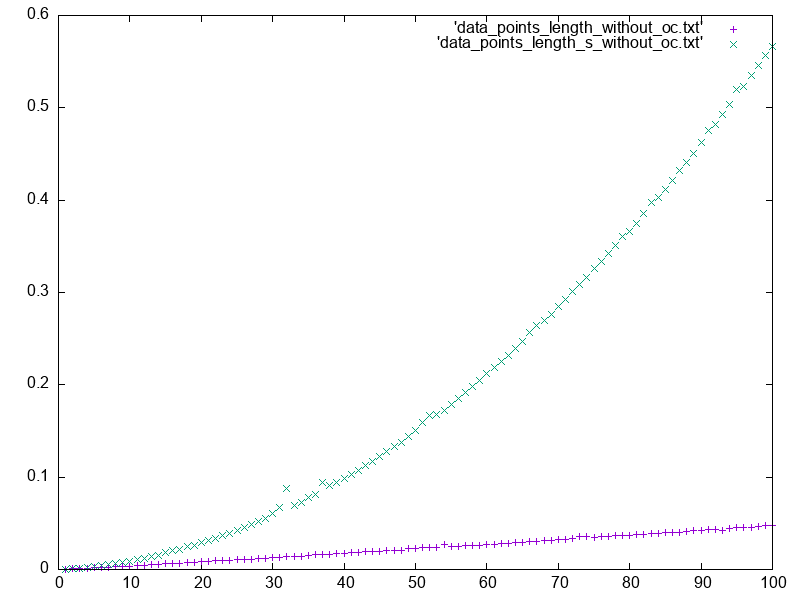
\includegraphics[width=6cm,height=5cm]{lengths_without_oc.png}
    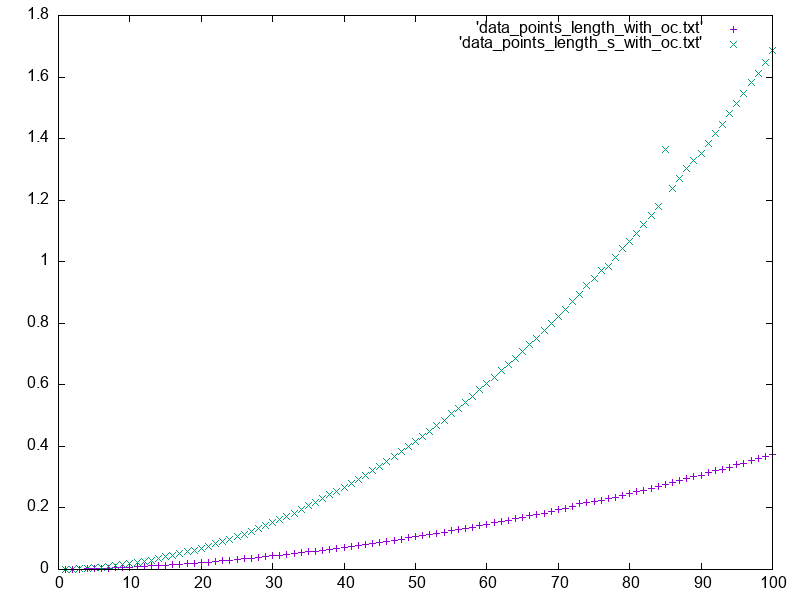
\includegraphics[width=6cm,height=5cm]{lengths_with_oc.png}
  \caption{Time (in seconds) of the search for the relations \lstinline|length$^o$| (purple) and \lstinline|length$_d^o$|} (green) depending on the lentgh of the list.
  Left: without occurs check.
  Right: with occurs check.
  \label{fig:length_plots}
\end{figure}

As a motivative example, consider two implementations of a standard recursive relation calculating the length of a list (see \figureword~\ref{fig:length_implementations}). They differ only in the
orders of conjuncts. Although the \lstinline|length$_d^o$| relation can be seen as a more direct definition of a function as a relation (all steps of usual length evaluation written up in order),
it is well-known that the \lstinline|length$^o$| with the recursive call in the end is much faster when running this relation backward (in fact, the search diverges if we
run \lstinline|length$_d^o$| backward, while for \lstinline|length$^o$| it terminates). What is less known and what we find more unexpected is the fact that if we run both relations
forward (specifying the list and asking for the length) \lstinline|length$^o$| is still much faster than \lstinline|length$_d^o$|, although they perform the same number of unifications. You can see the comparative time of the search in \figureword~\ref{fig:length_plots}. The difference is even
more staggering if we switch off occurs checks in unifications. It's OK because for simple queries like this occurs checks never violated. In the same \figureword~\ref{fig:length_plots} you can see that
the \emph{asymptotic complexity} becomes different in this case: it is linear for \lstinline|length$^o$| and quadratic for \lstinline|length$_d^o$|.

After investigating the execution for this example in detail we found that the difference is caused not by unifications but by the process of \emph{scheduling} of goals during the search.
During the execution of a program in \mK a lazy structure is build that decomposes the goals into unifications, performs these unifications in a certain order, and passes the results
appropriately. For the \lstinline|length$_d^o$| relation this structure becomes linear in size just because of the order in conjunctions and increases the time of
scheduling significantly. This kind of effect is hard to predict and measure without a formal model for performance in \mK.

This paper presents such a model. We study evaluation in a specific (canonical) implementation of \mK with goals evaluated to lazy streams in program-written order, but we rely only on the basic principles of implementation of \mK, so the model should be easily addoptable for a large class of regular implementations. We state that the total time of the search in \mK breaks into three separate parts: the time of scheduling ($T_s$) that breaks the evaluation into a sequence of
unifications, the time required to perform these unifications, and the time of reifications ($T_r$) that reconstruct the result in an expected form in the end. The time of unifications can be further
divided into the time of occurs checks ($T_{occ}$) during the unification and the time ($T_{uni}$) of the rest of the unification algorithm (this division will help us to see how large
is the part of the total time that occurs check, which often can be omitted, takes). So the total time of the search can be calculated as the sum of four components:

\[ T = T_s + T_{uni} + T_{occ} + T_r \]

We show how these components can be estimated and compared to each other in terms of asymptotics. The scheduling time complexity can be measured precisely since we link it to a specific value which we
call \emph{scheduling factor}, defined in terms of existing formal semantics of \mK (we recall the existing formal descriptions of \mK in \sectionword~\ref{sec:background}) and can be calculated using
a number of equations (\sectionword~\ref{sec:scheduling}). The other time components are hard to estimate precisely in general, as they are connected to the unification process, but we identify two
criteria that determine a wide range of cases for which these time components can be estimated easily (\sectionword~\ref{sec:uni-rei}). These separate methods for estimation of
different components of the time of the search can be put together in one approach for calculating manually the time complexity for a given query to a recursive relation (if this query satisfies the stated
criteria) using the principles of symbolic execution (\sectionword~\ref{sec:symbolic}). We then show the applicability of our method by applying it for a number of realistic \mK relations (\sectionword~\ref{sec:evaluation}).

\section{\mK: Syntax and Semantics}
\label{sec:background}

%In this section we recollect some known formal descriptions for \mK language that will be used as a basis for our development.
%Specifically, we restate the syntax of core language and the operational semantics for program evaluation.
%The descriptions here are taken from~\cite{CertifiedSemantics} (with a few non-essential adjustments for presentation purposes) to make
%the paper self-contained, more details and explanations can be found there.

\begin{figure}[t]
\centering
\[
\begin{array}{ccll}
  \mathcal{C} & = & \{C_i^{k_i}\} & \mbox{constructors} \\
  \mathcal{T}_X & = & X \cup \{C_i^{k_i} (t_1, \dots, t_{k_i}) \mid t_j\in\mathcal{T}_X\} & \mbox{terms over the set of variables $X$} \\
  \mathcal{D} & = & \mathcal{T}_\emptyset & \mbox{ground terms}\\
  \mathcal{X} & = & \{ x, y, z, \dots \} & \mbox{syntactic variables} \\
  \mathcal{A} & = & \{ x^?, y^?, z^? \dots \} & \mbox{logic variables} \\
  \mathcal{R} & = & \{ R_i^{k_i}\} &\mbox{relational symbols with arities} \\[2mm]
  \mathcal{G} & = & \mathcal{T_X}\equiv\mathcal{T_X}   &  \mbox{equality} \\
              &   & \mathcal{G}\wedge\mathcal{G}     & \mbox{conjunction} \\
              &   & \mathcal{G}\vee\mathcal{G}       &\mbox{disjunction} \\
              &   & \mbox{\lstinline|fresh|}\;\mathcal{X}\;.\;\mathcal{G} & \mbox{fresh variable introduction} \\
              &   & R_i^{k_i} (t_1,\dots,t_{k_i}),\;t_j\in\mathcal{T_X} & \mbox{relational symbol invocation} \\[2mm]
  \mathcal{S} & = & \{R_i^{k_i} = \lambda\;x_1^i\dots x_{k_i}^i\,.\, g_i;\}\; g & \mbox{specification}
\end{array}
\]
\caption{The syntax of \mK}
\label{fig:syntax}
\end{figure}

The syntax of core \mK is shown in Fig.~\ref{fig:syntax}. 
All data is presented using terms $\mathcal{T}_X$ built from a fixed set of constructors $\mathcal{C}$ with known arities and variables
from a given set $X$.
We parameterize the terms with an alphabet of variables since in the semantic description we will need \emph{two} kinds of variables:
\emph{syntactic} variables $\mathcal{X}$, used for bindings in the definitions, and \emph{logic} variables $\mathcal{A}$, which are
introduced and unified during the evaluation.

There are five types of goals: unification of two terms, conjunction and disjunction of goals
%(the ``\lstinline|conde|'' operator from the canonical versions of \mK, split in the two for simplicity),
fresh logic variable introduction, and invocation of some relational definition. For the sake of brevity, in code snippets, we abbreviate
immediately nested ``\lstinline|fresh|'' constructs into the one, writing ``\lstinline|fresh $x$ $y$ $\dots$ . $g$|'' instead of
``\lstinline|fresh $x$ . fresh $y$ . $\dots$ $g$|''. The \emph{specification} $\mathcal{S}$ consists of a set of relational definitions and a top-level goal.
A top-level goal represents a search procedure that returns a stream of substitutions for the free variables of the goal.
%The language we consider is first-order, as goals can not be passed as parameters, returned, or constructed at runtime.

During the evaluation of \mK program an environment, consisting of a substitution for logic variables and a counter of allocated logic
variables, is threaded through the computation and updated in every unification and fresh variable introduction.
The substitution in the environment at given point and given branch of evaluation contains all the information about relations between
the logical variables at this point. Hereafter we refer to the substitution in the environment at given point as ``current substitution''
in informal explanations.
Different branches are combined via \emph{interleaving search} procedure~\cite{InterleavingSearch}.
The answers for a given query are extracted from the final environments (they are the values of the queried variables in the final environment substitution).

This search procedure is formally described by operational semantics in the form of a labeled transition system.
This semantics corresponds to the canonical implementation of interleaving search. 

\begin{figure}[t]
\centering
\[
\begin{array}{ccllcccll}
  \Sigma & = & \mathcal{A} \to \mathcal{T}_\mathcal{A} & \mbox{substitutions} &\qquad\qquad&        S & = & \taskst{\mathcal{G}}{E} & \mbox{task} \\
       E & = & \Sigma \times \mathbb{N}              & \mbox{environments}  &\qquad\qquad&          &   & S \oplus S              & \mbox{sum} \\
         &   &                                       &                      &\qquad\qquad&          &   & S \otimes \mathcal{G}   & \mbox{product} \\
%         &   &                                       &                      &\qquad\qquad&  \hat{S} & = & \diamond \; \mid \; S   & \mbox{states} \\
       L & = & \circ \; \mid \; E      & \mbox{labels}        &\qquad\qquad&  \hat{S} & = & \diamond \; \mid \; S   & \mbox{states} \\
%         &   &                                       &                      &\qquad\qquad&        L & = & \circ \; \mid \; E      & \mbox{labels} 
\end{array}
\]
\caption{States and labels in the LTS for \mK}
\label{fig:operanional_semantics_states_labels}
\end{figure}

The form of states and labels in the transition system is defined in \figureword~\ref{fig:operanional_semantics_states_labels}.
Non-terminal states $S$ have a tree-like structure with intermediate nodes corresponding to partially evaluated conjunctions
(``$\otimes$'') or disjunctions (``$\oplus$'').
A leaf in the form $\taskst{g}{e}$ determines a task to evaluate a goal $g$ in an environment $e$. For a conjunction node, its right child
is always a goal since it cannot be evaluated unless some result is provided by the left conjunct.
We also need a terminal state $\diamond$ to represent the end of the evaluation.
The label ``$\circ$'' is used to mark those steps which do not provide an answer; otherwise, a transition is labeled by an updated
environment.

\begin{figure*}[h]
  \renewcommand{\arraystretch}{1.6}
  \[
  \begin{array}{crcr}
    \multicolumn{3}{c}{\taskst{t_1 \equiv t_2}{(\sigma, n)} \xrightarrow{\circ} \Diamond , \, \, \nexists\; mgu\,(t_1 \sigma, t_2 \sigma)} &\ruleno{UnifyFail} \\
    \multicolumn{3}{c}{\taskst{t_1 \equiv t_2}{(\sigma, n)} \xrightarrow{(mgu\,(t_1 \sigma, t_2 \sigma) \circ \sigma),\, n)} \Diamond} & \ruleno{UnifySuccess} \\
    \multicolumn{3}{c}{\taskst{\mbox{\lstinline|fresh|}\, x\, .\, g}{(\sigma, n)} \xrightarrow{\circ} \taskst{g\,[\bigslant{\alpha_{n + 1}}{x}]}{( \sigma, n + 1)}} & \ruleno{Fresh} \\
    \multicolumn{3}{c}{\dfrac{R_i^{k_i}=\lambda\,x_1\dots x_{k_i}\,.\,g}{\taskst{R_i^{k_i}\,(t_1,\dots,t_{k_i})}{e} \xrightarrow{\circ} \taskst{g\,[\bigslant{t_1}{x_1}\dots\bigslant{t_{k_i}}{x_{k_i}}]}{e}}} & \ruleno{Invoke}\\[3mm]
    \taskst{g_1 \lor g_2}{e} \xrightarrow{\circ} \taskst{g_1}{e} \oplus \taskst{g_2}{e} & \ruleno{Disj} &
    \taskst{g_1 \land g_2}{e} \xrightarrow{\circ} \taskst{g_1}{e} \otimes g_2 & \ruleno{Conj} \\    
    \dfrac{s_1 \xrightarrow{\circ} \Diamond}{(s_1 \oplus s_2) \xrightarrow{\circ} s_2} & \ruleno{DisjStop} &
    \dfrac{s_1 \xrightarrow{e} \Diamond}{(s_1 \oplus s_2) \xrightarrow{e} s_2} & \ruleno{DisjStopAns}\\
    \dfrac{s \xrightarrow{\circ} \Diamond}{(s \otimes g) \xrightarrow{\circ} \Diamond} &\ruleno{ConjStop} &
    \dfrac{s \xrightarrow{e} \Diamond}{(s \otimes g) \xrightarrow{\circ} \taskst{g}{e}}  & \ruleno{ConjStopAns}\\
    \dfrac{s_1 \xrightarrow{\circ} s'_1}{(s_1 \oplus s_2) \xrightarrow{\circ} (s_2 \oplus s'_1)} &\ruleno{DisjStep} &
    \dfrac{s_1 \xrightarrow{e} s'_1}{(s_1 \oplus s_2) \xrightarrow{e} (s_2 \oplus s'_1)} &\ruleno{DisjStepAns}\\
    \dfrac{s \xrightarrow{\circ} s'}{(s \otimes g) \xrightarrow{\circ} (s' \otimes g)} &\ruleno{ConjStep} &
    \dfrac{s \xrightarrow{e} s'}{(s \otimes g) \xrightarrow{\circ} (\taskst{g}{e} \oplus (s' \otimes g))} & \ruleno{ConjStepAns} 
  \end{array}
  \]
  \caption{Operational semantics of interleaving search}
  \label{fig:operanional_semantics_rules}
\end{figure*}

The transition rules are shown in Fig.~\ref{fig:operanional_semantics_rules}. The introduced transition system is completely deterministic,
therefore a derivation sequence for a state $s$ determines a certain \emph{trace}~--- a sequence of states and labeled transitions between
them. It may be either finite (ending with the terminal state $\Diamond$) or infinite. We will denote by $\trs{s}$ the sequence of states in
the trace for initial state $s$ and by $\tra{s}$ the sequence of answers in the trace for initial state $s$. The sequence $\tra{s}$ corresponds
to the stream of answers in the reference \mK implementations.

In the following we essentially rely on the following property of leaf states:

\begin{definition}
  A leaf state $\inbr{g, \sigma, n}$ is well-formed iff $\fv{g}\cup\Dom\,(\sigma)\cup\VRan\,(\sigma)\subseteq\{\alpha_1,\dots,\alpha_n\}$, where
  $\fv{g}$ denotes the set of free variables in a goal $g$, $\Dom\,(\sigma)$ and $\VRan\,(\sigma)$~--- the domain of a substitution $\sigma$ and
  a set of all free variables in its image respectively.
\end{definition}

This definition is in fact an instance of a more general definition of well-formedness for all states, introduced in~\cite{CertifiedSemantics}, where it is
proven that the initial state is well-formed and any transition from a well-formed state results in a well-formed one.

Besides operational semantics we will make use of a denotational one analoguous to the least Herbrand model. For a goal $g$ its denotational semantics $\sembr{g}$ is
treated as a $n$-ary relation on the set of all ground terms, where each ``dimension'' corresponds to some free variable in $g$. For example,
$\sembr{\lstinline|append$^o$ $\;\alpha\;\beta\;\gamma$|}$ is a set of all triplets of ground lists, in which the third component is a
concatenation of the first two. The concrete description of the denotational semantics is given in~\cite{CertifiedSemantics} as well as the proof of
the soundness and completeness of the operational semantics w.r.t. to the denotational one.

Finally, we explicitly enumerate all the restrictions required by our method to work:

\begin{itemize}
\item All relations habe to be in DNF (disjunctions of conjunctions of equalities or invocations);
\item We only consider goals which converge with a finite number of answers;
\item All answers have to be ground (\emph{groundness} condition);
\item All answers have to be unique (\emph{answer uniqueness} condition).
\end{itemize}

\section{Scheduling Complexity}
\label{sec:scheduling}

In this section we define a specific value to estimate the scheduling time and derive some equations to calculate this value for a given \emph{semantic
state}. However, our ultimate goal is to provide a complexity estimation for a given goal (\emph{query}). This problem will be addressed in Section~\ref{sec:symbolic},
in which we will make use of recurrent equations presented here.

We may notice that operational semantics described in the previous section can be used to calculate the exact number of elementary scheduling steps.
Our first idea is to take the number of states $d\,(s)$ in the finite trace for a given state $s$:

\[ d\,(s) \; \eqdef \; | \trs{s} |  \]

However, it turns out, that this value alone does not provide an accurate scheduling complexity estimation. The reason is that some
elementary steps in the semantics are not elementary in existing implementations. Namely, a careful analysis discovers that
each semantic step involves a navigation to the leftmost leaf of the state which in implementations corresponds to multiple elementary actions,
which number is proportional to the length of the leftmost branch of the state in question. Here we provide an \emph{ad-hoc} definition for this value, $t\,(s)$,
which we call the \emph{scheduling factor}:

\[
t\,(s) \eqdef \sum\limits_{s_i \in \trs{s}} lh\,(s_i) 
\]

where

\[
\begin{array}{rcl}
 lh\,(\taskst{g}{e})  &\eqdef& 1 \\
 lh\,(s_1 \oplus s_2) &\eqdef& lh\,(s_1) + 1 \\
 lh\,(s \otimes g)    &\eqdef& lh\,(s) + 1 \\
\end{array}
\]

In the rest of the section we state a number of lemmas providing estimations for these two values. The proofs for the lemmas (when omitted) can be
found in Appendix~\ref{sec:appendix}.

The first lemma provides a fundamental relation between these two~--- $d$ and $t$,~--- estimations for the scheduling complexity:

\begin{lemma}
\label{lem:d_t_relation}
 $d\,(s) \le t\,(s) \le d^2\,(s)$ for any state $s$.
\end{lemma}
\begin{proof}
  Follows immediately from the definitions of the estimated values and the fact that the height of a state increases by at most $1$ at each step.\qed
\end{proof}

Our next goal is to derive recurrent equations which would relate the scheduling complexity for states to the scheduling complexity for their
(immediate) substates. It turns out that to come up with such equations both $t$ and $d$ values have to be estimated simultaneously.  


% We take scheduling factor $t\,(s)$ as a value that determines the scheduling complexity $T_s$, but we will also need to calculate $d\,(s)$ as it will be used in the equations for $t\,(s)$. 

%In $\oplus$-states the substates are evaluated separately, one step at a time for each substate,
%so the total number of semantic steps is just a sum.
%However, for the scheduling factor, there is an extra summand since the heights of the states in
%the trace becomes bigger (by one additional $\oplus$-node on the top).
%This additional node exists in the trace until one of the substates is evaluated completely, so the
%scheduling factor is increased by the number of steps before such an event.
%So we have the following lemma.

The next lemma provides the equations for $\oplus$-states:

\begin{replemma}{lem:sum_measure_equations}
For any two states $s_1$ and $s_2$

\[
\begin{array}{rcl}
  d\,(s_1 \oplus s_2) &=& d\,(s_1) + d\,(s_2) \\
    t\,(s_1 \oplus s_2) &=& t\,(s_1) + t\,(s_2) + \costdisj{s_1}{s_2}
\end{array}
\]

where

\[ \costdisj{s_1}{s_2} = \min\,\{2\cdot d\,(s_1) - 1, 2\cdot d\,(s_2)\} \] 
\end{replemma}

Informally, for a state in the form $s_1 \oplus s_2$ the substates are evaluated separately, one step at a time for
each substate, so the total number of semantic steps is the sum of those for the substates. However, for the scheduling factor, 
there is an extra summand $\costdisj{s_1}{s_2}$ since the ``leftmost heights'' of the states in the trace are one node greater then those for the
original substates due to the introduction of one additional $\oplus$-node on the top. This additional node persists in the trace until the evaluation
of one of the substates comes to an end, so the scheduling factor is increased by the number of steps until that.

The next lemma provides the equations for $\otimes$-states:

\begin{replemma}{lem:times_measure_equations}
For any state $s$ and any goal $g$

\[
\begin{array}{rclr}
d\,(s \otimes g)  &=&  d\,(s) + \smashoperator[lr]{\sum\limits_{a_i \in \tra{s}}} d\,(\taskst{g}{a_i})& \qquad(\star) \\

 t\,(s \otimes g)  &=&  t\,(s) + \costconj{s}{g} + \smashoperator[lr]{\sum\limits_{a_i \in \tra{s}}} (t\,(\taskst{g}{a_i}) + \costdisj{\taskst{g}{a_i}}{(s'_i \otimes g)})&\qquad(\dagger)
\end{array}
\]

where 

\[
\begin{array}{rcl}
\costdisj{s_1}{s_2} & = & \min\,\{2\cdot d\,(s_1) - 1, 2\cdot d\,(s_2)\} \\
\costconj{s}{g} & = & d\,(s) \\
s'_i & = & \mbox{the first state in the trace for $s$ after} \\
 & & \mbox{a transition delivering the answer $a_i$} \\
\end{array}
\]
\end{replemma}

For the states of the form $s \otimes g$ the reasoning is the same, but the resulting equations are more complicated.
In $\otimes$-state the left substate is evaluated until an answer is found, which is then taken as
\emph{an environment} for the evaluation of the right subgoal.
Thus, in the equations for $\otimes$-states the evaluation times of the second goal \emph{for all
the answers} generated for the first substate are summed up. The evaluation of the right subgoal
in different environments are added to the evaluation of the left substate via the creation of
an $\oplus$-state, so for scheduling factor there is
an additional summand $\costdisj{\taskst{g}{a_i}}{s'_i}$ for each answer with $s'_i$ being the state
after discovering the answer.
There is also an extra summand $\costconj{s}{g}$ for the scheduling factor because of the
$\otimes$-node that increases the height in the trace, analogous to the one caused by
$\oplus$-nodes.
Note, $\otimes$-node is always placed immediately over the left substate so this
addition is exactly the number of steps for the left substate.

Unfolding costs definitions in $(\dagger)$ gives us a cumbersome formula which 
includes some intermediate states encountered during the evaluation. However, as ultimately
we are interested in an asymptotic estimations, we can approximate these costs up to a multiplicative constant.

First, we rewrite the equation $(\dagger)$ in the following form:

\[ t\,(s \otimes g)  =  t\,(s) + \smashoperator[lr]{\sum\limits_{a_i \in \tra{s}}} t\,(\taskst{g}{a_i}) + C\,(s \otimes g) \]

where

\[ C\,(s \otimes g) = \costconj{s}{g} + \smashoperator[lr]{\sum\limits_{a_i \in \tra{s}}} \costdisj{\taskst{g}{a_i}}{(s'_i \otimes g)} \]

Next, we need the following definition to handle corner cases.

\begin{comment}
\begin{definition}
Let $E$ be a set of environments, $g$~--- a goal. Then we call the value

\[
\alpha\,(g, E) = \argmax{e \in E} d\,(\taskst{g}{e})
\]

a \emph{pincipal environment}.
\end{definition}

In other words, $\alpha\,(g, E)$ is an element of $E$ which delivers the longest trace of $g$.
\end{comment}

\begin{definition}

For a set of natural numbers $S$

\[
\maxd \, S \eqdef
\begin{cases}
\max S,  & S \ne \emptyset \\
0, & S = \emptyset\\
\end{cases}
\]

\end{definition}

% With principal environment being defined we can prove the following lemma\footnote{We assume the following definition for 
% $h\,(x) = \Theta\,(f\,(x))$: \[\exists C_1, C_2 \in \mathcal{R^{+}}, \, \forall x : C_1 \cdot f\,(x) \le h\,(x) \le C_2 \cdot f\,(x) \]}:

Now we can state the following approximation\footnote{We assume the following definition for
$h\,(x) = \Theta\,(f\,(x))$: \[\exists C_1, C_2 \in \mathcal{R^{+}}, \, \forall x : C_1 \cdot f\,(x) \le h\,(x) \le C_2 \cdot f\,(x) \]}
for $C\,(s \otimes g)$.

\begin{replemma}{lem:times_costs_approximation}
\[
C\,(s \otimes g) =
\Theta\,(d\,(s) + \smashoperator[lr]{\sum\limits_{a_i \in \tra{s}}} d\,(\taskst{g}{a_i}) - \smashoperator{\maxd\limits_{a_i \in \tra{s}}} d\,(\taskst{g}{a_i}))	
\]
\end{replemma}

We can see that this approximation is very similar to the $(\star)$ except that here we exclude $d$ value for one of the answers from the sum (the maximal one). This difference
is essential and, as we will see later, it is in fact responsible for the difference in complexities for our motivation example.

Finally, as a result we have the following approximation for the scheduling factor of $\otimes$-states.

\begin{corollary}
\label{lem:otimes_t_approximation}
\[
 t\,(s \otimes g)  =  t\,(s) + \left({\sum\limits_{a_i \in \tra{s}}} t\,(\taskst{g}{a_i})\right) +
 \Theta\,(d\,(s) + \smashoperator[lr]{\sum\limits_{a_i \in \tra{s}}} d\,(\taskst{g}{a_i}) - \smashoperator{\maxd\limits_{a_i \in \tra{s}}} d\,(\taskst{g}{a_i}))	
\]
\end{corollary}









\begin{comment}

\textcolor{red}{\bf OR}

\begin{definition}
For two functions $f \colon X_1 \times \dots \times X_n \to \mathcal{R}$ and $g \colon X_1 \times \dots \times X_n \colon \mathcal{R} \to \mathcal{R}$ we say that $f(x_1,\, \dots,\, x_n) \sim_C g(x_1,\, \dots,\, x_n, C)$ if there exist two positive real constants $c^{low}$ and $c^{up}$ such that for all $(x_1,\, \dots,\, x_n) \in X_1 \times \dots \times X_n$, $g(x_1,\, \dots,\, x_n,\, c^{low}) \le f(x_1,\, \dots,\, x_n) \le g(x_1,\, \dots,\, x_n,\, c^{up})$.
\end{definition}

\begin{lemma}
\label{lem:prod_approximation}
For any state $s$ and any goal $g$
\[ 
\begin{array}{lcrl}

t\,(s \otimes g) & \lowupbound{1}{2} & & t\,(s) + (\displaystyle\sum\limits_{a_i \in \tra{s}} t\,(\taskst{g}{a_i})) + \\ 
& & C \cdot ( & d\,(s) + (\displaystyle\sum\limits_{a_i \in \tra{s}} d\,(\taskst{g}{a_i})) {\color{blue} - d\,(\taskst{g}{a_m})} ) 

\end{array} \]

where $a_m = \argmax{a_i \in \tra{s}} d(\taskst{g}{a_i})$
\end{lemma}

\textcolor{red}{\bf OR}

\begin{lemma}
\label{lem:prod_approximation}
\[ 
\begin{array}{lcrl}

t\,(s \otimes g) & \sim_C & & t\,(s) + (\displaystyle\sum\limits_{a_i \in \tra{s}} t\,(\taskst{g}{a_i})) + \\ 
& & C \cdot ( & d\,(s) + (\displaystyle\sum\limits_{a_i \in \tra{s}} d\,(\taskst{g}{a_i})) {\color{blue} - d\,(\taskst{g}{a_m})} ) 

\end{array} \]

where $a_m = \argmax{a_i \in \tra{s}} d(\taskst{g}{a_i})$
\end{lemma}

The blue addend is called ...

\end{comment}

\begin{comment}

One option is to go with the first argument of ``$\min$'' in $\costdisj{\taskst{g}{a_i}}{s'_i}$.
It should be a good approximation in the case when there are several answers passed to the second
goal and for none of them the number of steps surpasses the \emph{overall} number of steps for all
other answers (the second argument of ``$\min$'' will include the sum for the rest of the answers).

\begin{corollary}
\label{lem:prod_estimation_multiple_answers}
For any state $s$ and any goal $g$
\[ t\,(s \otimes g) \le t\,(s) + d\,(s) + \displaystyle\sum\limits_{a_i \in \tra{s}} (t\,(\taskst{g}{a_i}) + 2\cdot d\,(\taskst{g}{a_i}) \]
\end{corollary}

In the case when there is only one answer, however, we should rather go with the second argument of ``$\min$''. 

In this case the number of steps $d\,(s'_1 \otimes g)$ is equal to the number of steps $d\,(s'_1)$
since no more answers are produced, and we can approximate it by the length $d\,(s)$ of the whole
trace for $s$. 

\begin{corollary}
\label{lem:prod_estimation_single_answer}
  For any state $s$ and any goal $g$, if $\tra{s} = \{a\}$, then
  
\[ t\,(s \otimes g) \le t\,(s) + 3\cdot d\,(s) + t\,(\taskst{g}{a}) \]
\end{corollary}

Finally, since we estimate only up to a multiplicative constant (in particular, it does not matter by what constants we multiply the values of $d\,(\cdot)$ when calculating
the scheduling factor) we can derive from these results two compact scheduling time approximations for goals in the form of sequences of disjuncts/conjuncts.
These two approximations work regardless of the associativity/grouping of subformulas; thus a certain constant $c_k$, depending only on $k$, comes in.

For conjunctions, we have the following one.

\begin{lemma}
\label{lem:conjunction_metrics_calc}

Let $g = g_1 \land \dots \land g_k$ and let $A_i$ be a set of all answers that are passed to $g_i$ at some stage starting from some initial environment $e_0$

\[
\begin{array}{rcl}
A_1 &=& \{ e_0 \} \\
A_{i + 1} & = & \bigcup\limits_{a \in A_i} \tra{\taskst{g_i}{a}} 
\end{array}
\]

Then

\[
\begin{array}{rcl}
d\,(\taskst{g}{e}) &=& \displaystyle\sum\limits_{1 \le i \le k} \;\; \displaystyle\sum\limits_{a \in A_i} d\,(\taskst{g_i}{a}) \\
t\,(\taskst{g}{e}) &\le& \displaystyle\sum\limits_{1 \le i \le k} \;\; \displaystyle\sum\limits_{a \in A_i} t\,(\taskst{g_i}{a}) + c_k \cdot \displaystyle\sum\limits_{1 \le i \le k} \;\; \displaystyle\sum\limits_{a \in A_i} d\,(\taskst{g_i}{a}), \\
\end{array}
\]

In the case when all $A_i$ contain only one answer

\[
t\,(\taskst{g}{e}) \le \displaystyle\sum\limits_{1 \le i \le k} \;\; \displaystyle\sum\limits_{a \in A_i} t\,(\taskst{g_i}{a}) + c_k \cdot \displaystyle \sum\limits_{1 \le i \le k - 1} \;\; \displaystyle\sum\limits_{a \in A_i} d\,(\taskst{g_i}{a})
\]

\end{lemma}

When applying the estimation from corollary~\ref{lem:prod_estimation_multiple_answers} we have an extra summand in the form of the number of steps (multiplied by some constant) for all conjuncts.
The only exception is the case when every conjunct produces no more than one answer, then we can use the corollary~\ref{lem:prod_estimation_single_answer} everywhere instead and drop out the
additional number of steps for the last conjunct. Besides that, a constant number of steps is required to turn each conjunction into a $\otimes$-state, but we may integrate this extra constant into $c_k$.

For disjunctions, the lemma is the following one.

\begin{lemma}
\label{lem:disjunction_metrics_calc}

Let $g = g_1 \lor \dots \lor g_k$ and $1 \le l \le k$; then

\[
\renewcommand{\arraystretch}{1.5}
\begin{array}{rcl}
  d\,(\taskst{g}{e}) &\le& \displaystyle\sum\limits_{1 \le i \le k} d\,(\taskst{g_i}{e}) \\
  t\,(\taskst{g}{e}) &\le& \displaystyle\sum\limits_{1 \le i \le k} t\,(\taskst{g_i}{e}) + c_k\cdot \displaystyle\sum\limits_{\renewcommand{\arraystretch}{1}\begin{array}{c}1 \le i \le k \\ i \ne l\end{array}} d\,(\taskst{g_i}{e}).
\end{array}
\]

\end{lemma}

Roughly speaking, if we have a disjunct $g_m$ with a number of steps larger than all the steps for other disjuncts combined, then when applying lemma~\ref{lem:sum_estimation} we again will have an
extra summand in the form of the number of steps for all disjuncts except for the $g_m$ (it will always be the largest argument of ``$\min$''). But if we can drop out the \emph{largest}
the number of steps among disjuncts, we can also drop out any other instead, that's where arbitrary $l$ comes from. The case when there is no such $g_m$ has to be considered separately; it is simpler
since then all the numbers of steps are the same up to a multiplicative constant.

\end{comment}

\section{Unification and Reification Complexity}
\label{sec:uni-rei}

Syntactic unification of terms is a core operation for logic programming in whole and relational programming in particular.
However, the performance characteristics of conventional unification algorithms are rather hard to assess.
The known worst-case estimations say very little about the behavior of unification in \emph{practically important cases}, and, in
general, the very notion of ``practical importance'' is hard to formalize (which constitutes a generic problem for applied complexity as well).

The practical observations witness, that while the worst-case complexity for the conventional unification algorithm is exponential, in the majority of
cases met in practical logic programming the time for each unification problem instance throughout the program execution is linear or even constant on the size of the input.

%So the inner workings of unification are often neglected when estimating the performance of programs.

\mK has a distinctive way of implementing unification fitting in accordance with its ideology. First, since \mK aims at the purely functional implementation of an embedded logical
language it uses a triangular form of substitution~\cite{UnificationTheory} which allows a simple extension in a non-mutable fashion. Such substitutions are lazy in the sense that
they hold a partially substituted value for each variable, so to obtain a fully substituted value it may be necessary to apply a substitution repeatedly. In particular, a full
cycle of substitution application is needed at the end of the search to get the result for a queried variable. This process is called \emph{reification}. \mK uses the conventional Robinson's
algorithm for unification~\cite{RobinsonsAlgorithm}, adjusted for triangular substitutions~\cite{TRS}. Second, since \mK commits to adhere to logical consistency, by default it always
performs \emph{occurs checks} during the unification. Occurs check ensures that a binding being added into the substitution does not introduce any circularity, which is crucial for
establishing the soundness of unification results. However, being rarely violated, occurs check introduces a significant performance penalty, so some logical languages (such as \textsc{Prolog})
omit it.

In this section, we show how the complexity of unification can be assessed for many practical cases. Specifically, we present two dynamic criteria
for relational programs, under which every unification (omitting occurs check) in the program performs a constant number of basic operations. At the same
time, the occurs check, which complexity can be estimated separately, adds significant overhead to the execution time and often increases the asymptotic complexity.
A number of programs satisfying given tests and showing the impact of occurs check are listed in \sectionword~\ref{sec:evaluation}.

The actual time of unification depends on a concrete choice for a data structure to represent triangular substitutions (which are, abstractly, maps from integers to terms).
Therefore we parameterize our estimations by two values~--- $\lookuptime{\sigma}$ and $\addtime{\sigma}$,~--- which represent, respectively, the
worst-case asymptotic complexity for lookup and add operations w.r.t. to a substitution $\sigma$. The obvious candidate data structure is standard library maps
for a host language (and many implementations like \textsc{miniKanren}-with-symbolic-constraints and \textsc{OCanren} follow this recipe), which have logarithmic complexity for both operations,
so we expect this multiplier to be negligible. However, some implementations like \textsc{microKanren} use associative lists for simplicity of presentation (which have linear-time
lookup and constant-time addition complexities) or more complex data structures like random-access lists (which have a log-time lookup and average constant-time addition complexities)
so we keep this parameterization for the general case. The review of the performance of different date structures for triangular substitutions is given in~\cite{SubstDataStructs}.

The basic building block for the unification with triangular substitution is a \emph{walk} operation. This operation checks whether a given variable is mapped by a given substitution to a
term with a constructor at the top level. ``Walk'' continually looks up the substitution until a binding to a non-variable (in particular, no binding at all) is found. This
process can diverge only when there is a circular binding in the substitution, which, in turn, is excluded by the occurs check, so the substitutions are always consistent
in this sense~\cite{NominalUnificationWithTriangularSubstitutions}. Nevertheless ``walk'' can require a linear number (on the size of substitution) of lookups.
However, the variable-to-variable bindings occur rarely in practice and usually ``walk'' finds the required binding in one step. We can take the absence of variable-to-variable bindings
as our first criterion: for \emph{flat} substitutions (substitutions without such bindings) ``walk'' always makes only one lookup. We can relax this requirement by allowing a
constant number, independent of the input parameters of the topmost goal, of variable-to-variable bindings.

\begin{definition}
A substitution $\sigma$ is called \emph{constant-factor flat} if the number variable-to-variable bindings in $\sigma$ does not depend on the input parameters of the topmost goal.
\end{definition}

\begin{lemma}
If during the evaluation of a goal all substitutions are constant-factor flat, then the time of any walk during that evaluation on substitution $\sigma$ is $\lookuptime{\sigma}$.
\end{lemma}

The unification of two terms goes by the standard recursive descent. Each time a variable is encountered in a term being unified a ``walk'' step is performed, and if it ends up with
an unbound variable the occurs check is performed and, if succeeded, the substitution is extended. As the substitution grows during the process  the unified terms grow,
too, and the descent can go beyond the size of initial terms. But we argue that this happens not that often. For example, for a linear case (when any variable occurs in unified terms at
most once) the extensions of the substitution during the unification do not affect the unification in other branches, so the recursion will stop at the minimal height of the terms. 

\begin{lemma}
  Given two terms $t_1$ and $t_2$ and a current constant-factor flat substitution $\sigma$, if any variable occurs at most once in at most one of the terms $\{t_1 \sigma, t_2 \sigma\}$,
  then the time this unification takes, excluding occurs checks, is $\O\,(\min\,\{|t_1 \sigma|, |t_2 \sigma|\}) \cdot (\lookuptime{\sigma} + \addtime{\sigma})$.
\end{lemma}

In particular, if the size of one of those two terms does not depend on the input parameters (which is usually the case) the unification performs a constant number of basic operations.
This is our second criterion: linearity and constant size of one of the terms in every unification.

In the presence of occurs checks, however, we need to also go through every term we add in the substitution. This changes ``$\min$'' in the estimation above to ``$\max$'', making a huge
difference. Roughly speaking, in average the number of basic operations for every unification with occurs checks is approximately an average size of all terms unified in the program
(which is usually linear of the input). Therefore occurs checks add a huge time overhead for program execution in \mK, both for asymptotics (see \sectionword~\ref{sec:evaluation})
and for observable time~\cite{WillThesis}. This fact calls for an investigation into ways of going around occurs checks in \mK. Although simply omitting them is not an option for \mK,
there are other known approaches (mostly explored for \textsc{Prolog}), for example, static tests ensuring that occurs checks for a given program will never be violated~\cite{OccursCheckStaticTest}.
As far as we know, for now, there are no such solutions adopted for \mK.

For now, as we estimate the time of every individual unification it might be not clear how it relates to the estimations for the scheduling time. But since we consider cases in which unification
is relatively fast (constant number of basic operations), the number of unifications during an execution plays a more important role and it can be simply limited by the number of semantic
steps $d\,(s_{init}\,(input))$ (because every unification is a separate step in the semantics). Similarly, although the time of basic operations depends on the size of substitution in different points
of execution, logical variables for these bindings come either from the input (where there is usually a constant number of them) or from fresh variable allocations during the evaluation
(each of which is a separate step in the semantics). So the number of allocated logic variables (and therefore the maximum possible number of bindings) is limited by

\[
FV\,(input) + d\,(s_{init}\,(input))
\]

So, for example, for a usual case, when our two criteria are satisfied and the input contains a constant number of logic variables, for a standard implementation and without occurs checks
the total time of unifications $T_{uni}$ is $\O\,(d\,(s_{init}\,(input))\cdot \log d\,(s_{init}\,(input)))$

The time of reification $T_r$ can be estimated in the same way, since reification simply goes through the resulting term similarly to occur check. So in the case when the resulting
substitution is constant-factor flat, the number of basic operations for the reification is limited by the size of the output (multiplied by a constant). This time is usually dominated by the time of unification and scheduling, but not always (see examples in \sectionword~\ref{sec:evaluation}).

\section{Complexity Analysis via Symbolic Execution Schemes}
\label{sec:symbolic}

In the previous sections, we presented some methods to estimate the time complexity for scheduling and unification/reification (for the latter two only for some practical cases) in \mK, but they work
only for relational search in general, not for a specific relational program. In this section, we show how the latter task can be formulated and how those methods can be combined to solve
it using a notion of \emph{symbolic execution}.
Specifically, we add symbolic variables to \mK and use \emph{symbolic execution schemes} to build recursive inequalities for all components of our performance model.
These inequalities then can be solved to provide a symbolic representation for asymptotic estimations.

The application of symbolic execution for time complexity analysis is well-known and was explored for logic programming in particular~\cite{SymbolicExecutionForAnalysis}.
Usually, symbolic execution graphs are used to capture all the details of program execution which are significant for performance, and then the standard techniques for time (or other)
analysis of rewriting systems are applied. In contrast, we need symbolic execution graphs only as a neat representation of a general scheme of a relational search for a
given program and then bring in performance details using \emph{ad hoc} methods described in the previous sections. So we use a restricted version of a graph that corresponds
precisely to a body of a relation, not unfolding any relational calls. For this reason, we refer to them as ``symbolic execution schemes'' rather than ``symbolic execution graphs''.
This also means that we suppose that we know what answers any relational call in the program produces before we start the time complexity analysis.

\begin{figure}[t]
\begin{tabular}{p{6cm}p{6cm}}
\begin{lstlisting}[basicstyle=\small]
   prefix$^o$ = fun n p ->
     (p === Nil) \/
     (fresh (n' pt pti)
        (n === S(n')) /\
        (prefix$^o$ n' pt) /\
        (incr-list$^o$ pt pti) /\
        (p === Cons(S(O), pti))
     )
\end{lstlisting} &
\begin{lstlisting}[basicstyle=\small]
   incr_list$^o$ = fun a r ->
     ((a === Nil) /\ (r === Nil)) \/
     (fresh (h t tr)
        (a === Cons(h, t)) /\
        (r === Cons(S(h), tr)) /\
        (incr_list$^o$ t tr)
     )
\end{lstlisting}
\end{tabular}

\caption{Relational Prefixes Example}
\label{fig:prefixo_definition}
\end{figure}

To present the whole process in a clearer way we will go through it with a specific artificial example, in which almost all important details are presented. The example is a relational program
for generating all prefixes of a list \lstinline|$[1,\dots,n]$| (with numbers represented in Peano encoding with constructors \lstinline|O| and \lstinline|S|). Consider the
following creative recursive solution: we either take an empty prefix or take any prefix for the same task for $n - 1$ (if $n > 0$), increment all the elements, and add $1$ at the beginning.
The relation \lstinline|prefix$^o$| in \figureword~\ref{fig:prefixo_definition}, relating a number $n$ to some prefix $p$, follows this description directly. It uses a straightforwardly implemented relation \lstinline|incr-list$^o$|
that increments all numbers in a given list. This relation provides the required results: if we instantiate $n$ with some
Peano number and put a free logical variable for $p$ then $p$ will be bound to every prefix exactly once. It is an inefficient solution in many ways, but it is nice for presentation.

Now we want to estimate the time the search will take depending on a number we put as an input. To make our reasoning more precise we introduce the notion of \emph{symbolic variables}, which we will
denote with an overline ($\overline{a}, \overline{b}, \dots$) as opposed to the usual logic variables, which we will denote using a question mark ($a^{?}, b^{?}, \dots$). The symbolic
variables can be considered on two levels. At the level of symbolic execution, each symbolic variable in \mK stands for some ground term (a term without logic variables inside), but we do not know which
term exactly. At the metalevel, where we reason about the complexity of a program, a symbolic variable $\overline{x}$ stands for a representation of some object $x$ from metatheory (it can be a number, a
string, or a graph, for example) as a ground term, and we analyze how the program behaves depending on this object or some of its parameters. We will distinguish between these two levels throughout the
whole process of complexity analysis. For our example we consider the parametric query \lstinline{prefix$^o$ $\overline{k}$ $a^{?}$} with the first parameter instantiated by some number $k$
represented as a ground Peano term and second parameter left as a free logic variable, and ask how much time the search and its different stages will take depending on the value of $k$.

Our approach estimates the time complexity for some specific relational call with symbolic variables as arguments, not for a relation in general. We name every call we encounter to use these names in our
notations throughout the analysis (for example $pref = $ \lstinline{prefix$^o$ $\overline{k}$ $a^?$}). During the analysis we separately compute a number of factors for
the query that correspond to components of the overall time of the search in our model: the number of semantic steps $d^{pref}\,(k)$ and the scheduling factor $t_s^{pref}\,(k)$, which correspond to the number of semantic steps and the scheduling factor defined in \sectionword~\ref{sec:scheduling}, $t_{uni}^{pref}\,(k)$, which is the number of basic
operations performed during unifications in the execution of the call, excluding basic operations in occurs checks, $t_{occ}^{pref}(k)$, which is the number of basic operations performed during occurs checks, and $t_r^{pref}(k)$, which is the number of basic operations performed during the reification.

To achieve this, we build a symbolic execution scheme, mirroring the body of the examined relation, identify recursive calls, and reconstructing recursive inequalities for all the aforementioned factors
by using the estimations described in the previous sections. 
We put a number of restrictions for the examined relational call for our approach (however, as can be seen from the
\sectionword~\ref{sec:evaluation}, the huge variety of real examples satisfy them): the two criteria from \sectionword~\ref{sec:uni-rei} should be satisfied (which we can check using the symbolic execution, too), relations should be in disjunctive normal form.

We need to know also two extra pieces of information to perform the analysis for a given call. First, to  know how to proceed after recursive calls we need to know the answers that the calls produce.
We describe them by sets of substitutions binding all the logical variables in the query to terms, possibly containing fresh logic variables and symbolic variables, the latter we then specify in the metatheory (for example, $ANS^{pref}\,(k) = \{[a^? \gets \overline{p}] \mid \textit{$p$ is a prefix of the list \texttt{\lstinline|[$1$, .., $k$]|}} \} $). Second, we need to know all information for non-recursive relational calls
in the scheme (the values of all the complexity factors, produced answers, whether the requirements are satisfied). So we need to go and analyze these calls using the same approach
before we can examine the given call or reuse the information if we have already analyzed relevant call before. For this reason, we require the absence of mutual recursion in the examined calls
(it should be eliminated using standard techniques) and analyze them in the order of topological sorting. For $pref$ call we will need this information for the internal call $incr = $ \lstinline{incr-list$^o$ $\overline{l}$ $r^?$}, so we will analyze it first along the way.

% Here we just give it without details of the analysis (the analysis is much simpler than that for the $pref$ call): the requirements are satisfied,
% the answers are $ANS^{incr}(l) = \{[r^? \gets \overline{l'}] \; \mid \; length(l) = length(l') \land \forall i, \; l'[i] = l[i] + 1 \}$,
% and the complexity factors are as follows:

% \[
% \begin{array}{rcl}
%  d^{incr}\,(l) &\in& \O\,(len\,(l)) \\
%  t_s^{incr}\,(l) &\in& \O\,(len\,(l)) \\
%  t_{uni}^{incr}\,(l) &\in& \O\,(len\,(l)) \\
%  t_{occ}^{incr}\,(l) &\in& \O\,(len\,(l) \,\cdot\, size\,(l)) \\
%  t_{r}^{incr}\,(l) &\in& \O\,(size\,(l)) \\
%  \textit{where} && \\
%  size\,(l) &=& \sum_{x \in l} |\overline{x}| 
% \end{array} \]

\begin{figure}[t]
\begin{center}
\xymatrix{
     & \texttt{incr-list$^o$ $\overline{l}$ $r^?$} \ar[dl] \ar[dr] & \\
     \overline{l} \equiv \texttt{Nil} \ar[d]^{\{ [] \; \mid \; \overline{l} \;=\; \texttt{Nil} \}} & & \overline{l} \equiv \texttt{Cons($h^?$, $t^?$)} \ar[d]^{\{ [h^? \gets \overline{x}, t^? \gets \overline{l'}] \; \mid \; \overline{l} \;=\; \texttt{Cons($\overline{x}$, $\overline{l'}$)} \}} \\
     r^? \equiv \texttt{Nil} \ar[d]^{\{ [r^? \gets \texttt{Nil}] \}} & & r^? \equiv \texttt{Cons(S($\overline{x}$), $tr^?$)} \ar[d]^{\{ [r^? \gets \texttt{Cons(S($\overline{x}$), $tr^?$)}] \}} \\
     & & \texttt{incr-list$^o$ $\overline{l'}$ $tr^?$} \ar[d]^{ \{[tr^? \gets \overline{sl'}] \; \mid \; length(sl') = length(l') \land \forall i, \; sl'[i] = l'[i] + 1 \} } \\
     & & \\
}
\end{center}

\caption{Symbolic execution scheme for the $incr$ call}
\label{fig:incr_scheme}
\end{figure}

\begin{figure}[t]
\begin{center}
\xymatrix{
     & \texttt{prefix$^o$ $\overline{k}$ $p^?$} \ar[dl] \ar[dr] & \\
     p^? \equiv \texttt{Nil} \ar[d]^{\{ [p^? \gets \texttt{Nil}] \}} & & \overline{k} \equiv \texttt{S $n^?$} \ar[d]^{\{ [n^? \gets \overline{k'}] \; \mid \; \overline{k} \;=\; \texttt{S $\overline{k'}$} \}} \\
     & & \texttt{prefix$^o$ $\overline{k'}$ $pt^?$} \ar@2[d]^{ \{[pt^? \gets \overline{l}] \; \mid \; \textit{$l$ is a prefix of the list $[1..k']$} \} } \\
     & & \texttt{incr-list$^o$ $\overline{l}$ $pti^?$} \ar[d]^{ \{[pti^? \gets \overline{l'}] \; \mid \; length(l) = length(l') \land \forall i, \; l'[i] = l[i] + 1 \} } \\
     & & p^? \equiv \texttt{Cons (S(O), $\overline{l'}$)} \ar[d]^{ \{[p^? \gets \texttt{Cons (S(O), $\overline{l'}$)}] \} } \\
     & & \\
}
\end{center}

\caption{Symbolic execution scheme for the $pref$ call}
\label{fig:pref_scheme}
\end{figure}


The symbolic execution scheme for the $pref$ call is shown in \figureword~\ref{fig:pref_scheme} and the scheme for the internal call $incr$ is shown in \figureword~\ref{fig:incr_scheme}. A symbolic execution scheme shows unifications and internal relational calls evaluated during the search for the initial call and the answers that are threaded through the search. The initial call is at the top.
For simplicity we work only with the relations in disjunctive normal form, each disjunct is represented as a separate column on the scheme. The nodes of the column are
the unifications and relational calls in the given conjunct, they are written down sequentially in the same order as in the relation and connected by arrows. Arrows are
labeled with the description of a set of answers, produced by the previous node. This description is represented as a set of lists of bindings for logical variables by which the
substitution is extended, the generator of the set (the condition after the `$\mid$' symbol) is described in terms of metatheory. For the analysis we need to distinguish
cases when multiple answers are produced so we denote by a single arrow $\downarrow$ the sets that we know to have no more than one answer, and put a double arrow $\Downarrow$
in other cases. The answers produced by internal relational calls are given as a prerequisite for the analysis. The unifications may produce new substitutions for
both logic variables and symbolic variables. The definition of unification with both logic and symbolic variables is shown on \figureword~\ref{fig:symbolic_unification}.
Bindings for logical variables in the result are extensions of the substitution in the environment after this unification, and bindings for symbolic variables are conditions
for the objects in metatheory represented by these symbolic variables, under which we continue to execute the current branch. For example, the unification for $\overline{x} \equiv f\,(t_1, \dots, t_k)$ will succeed only for object $x$ such that its representation is $f\,(\overline{x_1}, \dots, \overline{x_k})$, where $\overline{x_i}$ are the representations which are the terms
unifiable with $t_i$. So we add bindings for symbolic variables to the generator of the set in the form of equalities. We apply bindings for both logic and symbolic variables in
all nodes after we get them to show the fully substituted values of terms.

%\begin{figure}[t]
%  \small
%\[
%\begin{array}{lll}
%  U(w^?, w^?) &= \epsilon & \\
%  U(w^?, t) &= \bot & \textit{if $w^? \in FV(t)$} \\
%  U(w^?, t) &= [w^? \gets t] & \textit{if $t \ne w^? \land w^? \not\in FV(t)$} \\
%  U(\overline{x}, w^?) &= [w^? \gets \overline{x}] &  \\
%  U(\overline{x}, \overline{y}) &= [\overline{x} \gets \overline{y}] &  \\
%  U(\overline{x}, f(t_1, \dots, t_k)) &= [\overline{x} \gets f(\overline{x_1}, \dots, \overline{x_k})] \circ U(\overline{x_1}, t_1) \circ \dots \circ  U(\overline{x_k}, t_k)  & \textit{where $\overline{x_i}$ are fresh}  \\
%  U(f(t_1, \dots, t_k), w^?) &= \bot & \textit{if $w^? \in FV(f(t_1, \dots, t_k))$} \\
%  U(f(t_1, \dots, t_k), w^?) &= [w^? \gets f(t_1, \dots, t_k)] & \textit{if $w^? \not\in FV(f(t_1, \dots, t_k))$} \\
%  U(f(t_1, \dots, t_k), \overline{x}) &= [\overline{x} \gets f(\overline{x_1}, \dots, \overline{x_k})] \circ U(t_1, \overline{x_1}) \circ \dots \circ U(t_k, \overline{x_k})  & \textit{where $\overline{x_i}$ are fresh}  \\
 % U(f(t_1, \dots, t_k), f(t'_1, \dots, t'_k)) &= U(t_1, t'_1) \circ \dots \circ U(t_k, t'_k)  & \\
 % U(f(t_1, \dots, t_k), g(t'_1, \dots, t'_{k'})) &= \bot  & \textit{if $f \ne g$} \\
%  
%\end{array}
%\]
%  \caption{Unification for terms with logic and symbolic variables; $t$ stands for an arbitrary term.}
%  \label{fig:symbolic_unification}
%\end{figure}

\begin{figure}[t]
  \small
\[
\begin{array}{lll}
  U(w^?, w^?) &= \epsilon & \\
  U(w^?, t) &= \bot & \textit{if $w^? \in FV(t)$} \\
  U(w^?, t) &= [w^? \gets t] & \textit{if $t \ne w^? \land w^? \not\in FV(t)$} \\
  U(t, w^?) &= U(w^?, t) & \textit{if $t$ is not a logic variable} \\
  U(\overline{x}, \overline{y}) &= [\overline{x} \gets \overline{y}] &  \\
  U(\overline{x}, f(t_1, \dots, t_k)) &= [\overline{x} \gets f(\overline{x_1}, \dots, \overline{x_k})] \circ U(\overline{x_1}, t_1) \circ \dots \circ U(\overline{x_k}, t_k)  & \textit{where $\overline{x_i}$ are fresh}  \\
  U(f(t_1, \dots, t_k), \overline{x}) &= U(\overline{x}, f(t_1, \dots, t_k))  \\
  U(f(t_1, \dots, t_k), f(t'_1, \dots, t'_k)) &= U(t_1, t'_1) \circ \dots \circ U(t_k, t'_k)  & \\
  U(f(t_1, \dots, t_k), g(t'_1, \dots, t'_{k'})) &= \bot  & \textit{if $f \ne g$} \\
  
\end{array}
\]
  \caption{Unification for terms with logic and symbolic variables; $t$ stands for an arbitrary term.}
  \label{fig:symbolic_unification}
\end{figure}

This scheme presents all the information we need to check the criteria and calculate the complexity of all the factors using the results from the previous sections.

\begin{enumerate}
\item To check that all substitutions are flat during the evaluation we need to know that all non-recursive internal calls satisfy this condition and to check that no variable-to-variable bindings are added during the evaluation of the body of the relation. To check this we can simply check that rhs of all bindings on arrows after unifications are not logical variables (then the value in the binding
necessarily has a constructor on the top-level).

If there are no recursive calls in the scheme, we can allow variable-to-variable bindings after substitutions, since there will be at most a constant number of them and substitutions will always be constant-factor flat.

The second criterion (linearity and constant size of one of the terms for every unification) we can easily check directly: for every unification on the scheme each logical variable should occur at most once and one of the terms should have no symbolic variables. We also need the criterion to be satisfied for all the internal calls.

For the calls $incr$ and $pref$ the both criteria are satisfied.

\item To estimate $d^{incr}\,(l)$ and $d^{pref}\,(k)$ we use lemmas \ref{lem:conjunction_metrics_calc} and \ref{lem:disjunction_metrics_calc}. Specifically, we just add the corresponding value for every internal call summed up for all the answers for which the call is executed, and also add a constant to handle the rest (unifications and fresh variable introductions). We know the value of $d^q\,(\dots)$ for every internal call $q$: for non-recursive internal calls we have the estimation up to a multiplicative constant from the previous analysis, for recursive internal calls it's just the value of the same function with a different argument.
  
So, for the $incr$ call we have:

\[ d^{incr}\,(l) \le C + \displaystyle\sum\limits_{\overline{l} \;=\; \texttt{Cons($\overline{x}$, $\overline{l'}$)}} d^{incr}\,(l') \]

Considering two cases when $l$ is empty and non-empty list we can simplify the inequality above into the following two:

\[
\begin{array}{lcl}
d^{incr}\,([]) &\le& C \\
d^{incr}\,(x : l') &\le& C + d^{incr}\,(l')
\end{array} \]

which we can easily solve and get $d^{incr}\,(l) \in \O\,(len\,(l))$.

And for the $pref$ call we have:

\[ d^{pref}\,(k) \le C + \displaystyle\sum\limits_{\overline{k} \;=\; \texttt{S $\overline{k'}$}} (d^{pref}\,(k') + \displaystyle\sum\limits_{\textit{$l$ is a prefix of the list $[1..k']$}} d^{incr}\,(l)) \]

Which we can rewrite and simplify again by considering two cases and substituting calculated complexity for $d^{incr}\,(l)$:

\[
\begin{array}{lcl}
d^{pref}\,(0) &\le& C \\
d^{pref}\,(k' + 1) &\le& C + d^{pref}\,(k') + \displaystyle\sum\limits_{i \in [0..k']} C \cdot i \\
            &\le& d^{pref}\,(k') + C \cdot k'^2 
\end{array} \]

From which we get $d^{pref}\,(k) \in \O\,(k^3)$.

\item For $t_s^{incr}\,(l)$ and $t_s^{pref}\,(k)$ we do basically the same using the same lemmas \ref{lem:conjunction_metrics_calc} and \ref{lem:disjunction_metrics_calc}. The difference is that for every internal call $q$ along with $t_s^q\,(\dots)$ we have to add $d^q\,(\dots)$
  multiplied by a constant (for recursive calls we use the complexity calculated at the previous step). There is a possible exception, however (identified in the lemmas): for one column that has only single arrows, we can omit additional $d^q\,(\dots)$ for the last call in the column (if the column ends with a call).
  By lemma~\ref{lem:disjunction_metrics_calc} we can pick any column, it might make difference only when this value $d^q\,(\dots)$ dominates all the other values. In particular, in the case when a relation has one recurisve call, if it is in the end of a conjunction we omit additional value $d^q\,(\dots)$ for this call, and when it is not in the end we can not omit this additional value (and can omit the additional value $d^q\,(\dots)$ for the last non-recursive call instead, which will be dominated by the value $t^q\,(\dots)$ for this call with a multiplicative factor anyway). This omission is precisely the reason for the change in complexity when the recursive call is moved to the end, like in the initial example of \lstinline|length$^o$| and \lstinline|length$_d^o$| relations in \sectionword~\ref{sec:intro}. Likewise, for $incr$ call we omit additional value $d^{incr}\,(l')$ for the recursive call and get the same inequality as the one for the number of steps:

\[ t_s^{incr}\,(l) \le C + \displaystyle\sum\limits_{\overline{l} \;=\; \texttt{Cons($\overline{x}$, $\overline{l'}$)}} t_s^{incr}\,(l') \]
 
So, $t_s^{incr}\,(l)$ is also in $\O\,(len\,(l))$.
 
In contrast, in $pref$ call the recursive call is not in the end, so we have additional value $d^{pref}(k')$ for it, which affects the resulting complexity:

  \[
\begin{array}{rclc}
  t_s^{pref}\,(k) & \le C + \displaystyle\sum\limits_{\overline{k} \;=\; \texttt{S $\overline{k'}$}} (& t_s^{pref}\,(k') & + \\
                &     & C \cdot d^{pref}(k') & + \\
                &     & \displaystyle\sum\limits_{\textit{$l$ is a prefix of the list $[1..k']$}} (t_s^{incr}\,(l) + C \cdot d^{incr}\,(l))) & \\
\end{array}
\]

After the simplification, we get the following two inequalities:

\[ \begin{array}{rcl}
t_s^{pref}\,(0) &\le& C \\
t_s^{pref}\,(k' + 1) &\le& C + t_s^{pref}\,(k') + C \cdot k'^3 + \displaystyle\sum\limits_{i \in [0..k']} (C \cdot i + C \cdot i) \\
                  &\le& t_s^{pref}\,(k') + C \cdot k'^3 
\end{array} \]

And after solving them we get $t_s^{pref}\,(k) \in \O\,(k^4)$.

\item To estimate $t_{uni}^{incr}\,(l)$ and $t_{uni}^{pref}\,(k)$ we just do the same summation, counting the number of unifications in the scheme and in the internal calls.

For $incr$ we have the following inequality:

\[ t_{uni}^{incr}\,(l) \le 1 + (\displaystyle\sum\limits_{\overline{l} \;=\; \texttt{Nil}} 1) + 1 + \displaystyle\sum\limits_{\overline{l} \;=\; \texttt{Cons($\overline{x}$, $\overline{l'}$)}} (1 + t_{uni}^{incr}\,(l') ) \]

The simplified version is the following:

\[ \begin{array}{lcl}
t_{uni}^{incr}\,([]) &\le& C \\
t_{uni}^{incr}\,(x : l') &\le& C + t_{uni}^{incr}\,(l') \\
\end{array} \]

And the result is $t_{uni}^{incr}\,(l) \in \O\,(len\,(l))$.

And for $pref$ we have the following inequality:

  \[
    t_{uni}^{pref}\,(k) \le 1 + 1 + \displaystyle\sum\limits_{\overline{k} \;=\; \texttt{S $\overline{k'}$}} (t_{uni}^{pref}\,(k') + \displaystyle\sum\limits_{\textit{$l$ is a prefix of the list $[1..k']$}} (t_{uni}^{incr}\,(l) + \displaystyle\sum\limits_{l': \; length(l) = length(l') \land \forall i, \; l'[i] = l[i] + 1} 1))
    \]

The simplified version is the following:

\[ \begin{array}{rcl}
t_{uni}^{pref}\,(0) &\le& C \\
t_{uni}^{pref}\,(k' + 1) &\le& C + t_{uni}^{pref}\,(k') + \displaystyle\sum\limits_{i \in [0..k']} (C \cdot i + 1) \\
&\le& t_{uni}^{pref}\,(k') + C \cdot k'^2
\end{array} \]

And the result is $t_{uni}^{pref}\,(k) \in \O\,(k^3)$.

\item To estimate $t_{occ}^{incr}\,(l)$ and $t_{occ}^{pref}\,(k)$ we just do the same summation, counting the sizes of rhs in bindings on arrows after every unification on the scheme and the same in the internal calls.

For $incr$ we have the following inequality:

\[ t_{occ}^{incr}\,(l) \le (\displaystyle\sum\limits_{\overline{l} \;=\; \texttt{Nil}} |\texttt{Nil}|) + \displaystyle\sum\limits_{\overline{l} \;=\; \texttt{Cons($\overline{x}$, $\overline{l'}$)}} (|\overline{x}| + size(l') + |\texttt{Cons(S($\overline{x}$), tr)}| + t_{occ}^{incr}\,(l') ), \]

where $size\,(l') = \displaystyle\sum\limits_{y \in l'} |\overline{y}|$.

The simplified version is the following:

\[ \begin{array}{lcl}
t_{uni}^{incr}\,([]) &\le& C \\
t_{uni}^{incr}\,(x : l') &\le& C + 2 |\overline{x}| + size(l') + t_{uni}^{incr}\,(l') \\
\end{array} \]

And the result is $t_{uni}^{incr}\,(l) \in \O\,(len\,(l) \cdot size\,(l))$.

And for $pref$ we have the following inequality:

%!!!!!!!!!!!!

\[ \begin{array}{c} t_{occ}^{pref}\,(k) \le C + \displaystyle\sum\limits_{\overline{k} \;=\; \texttt{S $\overline{k'}$}} (k' + t_{occ}^{pref}\,(k') + \displaystyle\sum\limits_{\textit{$l$ is a prefix of the list $[1..k']$}} (t_{occ}^{incr}\,(l) + \\ \displaystyle\sum\limits_{l': \; length(l) = length(l') \land \forall i, \; l'[i] = l[i] + 1} |\texttt{Cons (S(O), $\overline{l'}$)}|)) \end{array}  \]

The simplified version is the following.

\[ \begin{array}{rcl}
t_{occ}^{pref}\,(0) &\le& C \\
t_{occ}^{pref}\,(k' + 1) &\le& C + k' + t_{occ}^{pref}\,(k') + \displaystyle\sum\limits_{i \in [0..k']} (C \cdot i^3 + C \cdot i^2 + C) \\
\phantom{t_{occ}^{pref}\,(k' + 1)} &\le& t_{occ}^{pref}\,(k') + C \cdot k'^4
\end{array} \]

And the result is $t_{occ}^{pref}\,(k) \in \O\,(k^5)$.

\item Finally, to estimate $t_{r}^{pref}\,(k)$ we just sum the sizes of all answers from $ANS^{pref}\,(k)$.

$t_{r}^{pref}\,(k) = \displaystyle\sum\limits_{\textit{$l$ is a prefix of the list $[1..k]$}} size(l) \le \displaystyle\sum\limits_{i \in [0..k]} C \cdot i^2 \le C \cdot k^3$

So $t_{r}^{pref}\,(k) \in \O\,(k^3)$.

\end{enumerate}

This way we get the complexity for all the components of the search. Now we can combine them to get the complete estimation. To get the time related to the unification we should
multiply $t_{uni}^{pref}$, $t_{occ}^{pref}$, $t_r^{pref}$ by a multiplier $(\lookuptime{|\sigma|} + \addtime{|\sigma|}))$ which we can estimate
by $(\lookuptime{d^{pref}(k)} + \addtime{d^{pref}(k)}))$. So, for example, for an implementation with standard-library maps for substitutions the complete time of the
search for the call \lstinline{prefix$^o$ $\overline{k}$ $a^?$} is $\O\,(k^4 + k^3 \log k + k^5 \log k + k^3 \log k) = \O\,(k^5 \log k)$ with occurs checks and
$\O\,(k^4 + k^3 \log k + k^3 \log k) = \O\,(k^4)$ without.

%\begin{figure}[t]
%\centering
%\includegraphics{graph2.pdf}
%\caption{The Second Set of Benchmarks}
%\label{eval:second}
%\end{figure}

\section{Performance Evaluation}
\label{sec:evaluation}

One of our initial goals was to evaluate, what performance impact would choosing OCaml as a host language make. In addition we spent some 
efforts in order to implement \miniKanren in an efficient, tagless manner, and, of course, the outcome of this decision also has to be 
measured. For comparison we took faster-miniKanren\footnote{\url{https://github.com/webyrd/faster-miniKanren}}~--- a full-fledged 
\miniKanren implementation for Scheme/Racket. It turned out that faster-miniKanren implements a number of optimizations~\cite{WillThesis, Optimizations} 
to speedup the search; moreover, the search order in our implementation initially was a little bit different. In order to make the comparison
fair, we additionally implemented all these optimizations and adjusted the search order to exactly coincide with 
what faster-miniKanren does.

\begin{figure}[t]
\centering
\includegraphics[scale=0.4]{graph.png}
\caption{The Results of the Performance Evaluation}
\label{eval}
\end{figure}

\FloatBarrier 

For the set of benchmarks we took the following problems:

\begin{itemize}
%\item \textbf{sorto, permo}~--- sorting and permutation for lists of Peano numbers (shown as example in Section~\ref{sec:examples}).
%The concrete tests are the sorting of the list \lstinline{[3; 2; 1; 0]} and taking all permutations of the list \lstinline{[0; 1; 2; 3; 4; 5; 6; 7]}.
\item \textbf{pow, logo}~--- exponentiation and logarithm for integers in binary form. The concrete tests relationally computed
$3^5$ (which in 243) and $log_3 243$ (which is, conversely, 5).
\item \textbf{quines, twines, trines}~--- self/co-evaluating program synthesis problems from~\cite{Untagged}. The
concrete tests took the first 100, 15 and 3 answers for these problems respectively.
\end{itemize}

%Since the last bundle of benchmarks uses disequality constraints (and, hence, $\mu$Kanren is ruled out) we
%split all benchmarks into two sets.

The evaluation was performed on a desktop computer with Intel Core i7-4790K CPU @ 4.00GHz processor and 16GB of memory.
For OCanren \mbox{ocaml-4.04.0+frame_pointer+flambda} was used, for faster-miniKanren~--- Chez~Scheme~9.4.1.
All benchmarks were ran in the natively compiled mode ten times, then average user time was taken. The results of the evaluation
are shown on Figure~\ref{eval}. The whole evaluation repository with all scripts and detailed description is accessible 
from \lstinline{GitHub}\footnote{\url{https://github.com/Kakadu/ocanren-perf}}.

The first conclusion, which is rather easy to derive from the results, is that the tagless approach indeed matters. Our initial
implementation did not show essential speedup in comparison even with $\mu$Kanren (and was even \emph{slower} on the logarithm
and permutations benchmarks). The situation was improved drastically, however, when we switched to the tagless version.

Yet, in comparison with faster-miniKanren our implementation is still lagging behind. We can conclude, that the optimizations, 
used in Scheme/Racket version, have a different impact in the OCaml case; we save this problem for future research.


\section{Conclusion}
\label{conclusion}

We presented an improvement of a search strategy for relational programming, which is aimed at
improving refutationally completeness. We've proven, that in the case of a finite number of 
answers our modification is a strict improvement over the original strategy. Our evaluation 
shows, that w.r.t. the improved search many practically important refutationally incomplete 
queries became refutationally complete; in addition in a number of cases the performance was greatly 
improved since our modification, as a side effect, causes the search to choose more 
``optimistic'' branches. 

We can identify the following directions for future work. 

First, we believe, that our result on refutational improvement for a finite number of answers 
can be extended to the general case as well (note, in our current development we did not make 
any use of the \emph{completeness} property of miniKanren search). For this, we would also need 
another, more general, semantics. 

Another direction is extending the language with disequality constraints. Our evaluation has 
shown, that disequality constraints do not compromise our improvement in all user benchmarks, 
but we do not have a proof, that they are indeed harmless.

Next, we are working on a certified proof of the main theorem in Coq.

Finally, our practical evaluation is performed only for a prototype. 
We consider the embedding of our improvement in a full-fledged implementation to be
an important task.

%%
%% The acknowledgments section is defined using the "acks" environment
%% (and NOT an unnumbered section). This ensures the proper
%% identification of the section in the article metadata, and the
%% consistent spelling of the heading.
%%\begin{acks}

%%\end{acks}

%%
%% The next two lines define the bibliography style to be used, and
%% the bibliography file.
\bibliographystyle{splncs04}
\bibliography{main}

%%
%% If your work has an appendix, this is the place to put it.
\appendix

\section{Definitions of the evaluated relations}
\label{sec:examples_definitions}

Here are the definitions of the \mK relations we used for evaluation. Different queries to the same relation may require different orders in conjunctions.

\begin{enumerate}

\item Comparison of Peano numbers

Definition:

\begin{lstlisting}[basicstyle=\small]
   le$^o$ = fun x y ->
     (x === O) \/
     (fresh (x' y')
        (x === S(x')) /\
        (y === S(y')) /\
        (le$^o$ x' y')
     )
\end{lstlisting}

For queries:

\begin{itemize}
\item[-] \lstinline{le$^o$ $\overline{n}$ $\overline{m}$}

\item[-] \lstinline{le$^o$ $x^?$ $\overline{m}$}

\item[-] \lstinline{le$^o$ $\overline{n}$ $y^?$}
\end{itemize}


\item Sum of Peano numbers

Definition:

\begin{lstlisting}[basicstyle=\small]
   plus$^o$ = fun x y r ->
     ((x === O) /\ (y === r)) \/
     (fresh (x' r')
        (x === S(x')) /\
        (r === S(r')) /\
        (plus$^o$ x' y r')
     )
\end{lstlisting}

For queries:

\begin{itemize}
\item[-] \lstinline{plus$^o$ $\overline{n}$ $\overline{m}$ $r^?$}

\item[-] \lstinline{plus$^o$ $\overline{n}$ $y^?$ $\overline{k}$}

\item[-] \lstinline{plus$^o$ $x^?$ $y^?$ $\overline{k}$}
\end{itemize}


\item Product of Peano numbers

Definition \#1:

\begin{lstlisting}[basicstyle=\small]
   mult$^o$ = fun x y r ->
     ((x === O) /\ (r === O)) \/
     (fresh (x' r')
        (x === S(x')) /\
        (mult$^o$ x' y r') /\
        (plus$^o$ r' y r)
     )
\end{lstlisting}

For query:

\begin{itemize}
\item[-] \lstinline{mult$^o$ $\overline{n}$ $\overline{m}$ $r^?$}
\end{itemize}

Definition \#2:

\begin{lstlisting}[basicstyle=\small]
   mult$^o$ = fun x y r ->
     ((x === O) /\ (r === O)) \/
     (fresh (x' r')
        (x === S(x')) /\
        (plus$^o$ r' y r) /\
        (mult$^o$ x' y r')
     )
\end{lstlisting}

For queries:

\begin{itemize}
\item[-] \lstinline{mult$^o$ $x^?$ $\overline{m + 1}$ $\overline{k}$}

\item[-] \lstinline{mult$^o$ S($x^?$) S($y^?$) $\overline{k}$}
\end{itemize}


\item Length of a list

Definition \#1:

\begin{lstlisting}[basicstyle=\small]
   length$_d^o$ = fun a r ->
     ((a === Nil) /\ (x === O)) \/
     (fresh (h t r')
        (a === Cons(h, t)) /\
        (length$_d^o$ t r') /\
        (r === S(r'))
     )
\end{lstlisting}

For query:

\begin{itemize}
\item[-] \lstinline{length$_d^o$ $\overline{l}$ $r^?$}
\end{itemize}

Definition \#2:

\begin{lstlisting}[basicstyle=\small]
   length$^o$ = fun a r ->
     ((a === Nil) /\ (x === O)) \/
     (fresh (h t r')
        (a === Cons(h, t)) /\
        (r === S(r')) /\
        (length$^o$ t r')
     )
\end{lstlisting}

For queries:

\begin{itemize}
\item[-] \lstinline{length$^o$ $\overline{l}$ $r^?$}

\item[-] \lstinline{length$^o$ $a^?$ $\overline{n}$}
\end{itemize}


\item Incrementing all elements in a list

Definition:

\begin{lstlisting}[basicstyle=\small]
   incr_list$^o$ = fun a r ->
     ((a === Nil) /\ (r === Nil)) \/
     (fresh (h t tr)
        (a === Cons(h, t)) /\
        (r === Cons(S(h), tr)) /\
        (incr_list$^o$ t tr)
     )
\end{lstlisting}

For queries:

\begin{itemize}
\item[-] \lstinline{incr_list$^o$ $\overline{l}$ $r^?$}

\item[-] \lstinline{incr_list$^o$ $a^?$ $\overline{l}$}
\end{itemize}


\item Concatination of two lists

Definition:

\begin{lstlisting}[basicstyle=\small]
   append$^o$ = fun a b r ->
     ((a === Nil) /\ (b === r)) \/
     (fresh (h t tb)
        (a === Cons(h, t)) /\
        (r === Cons(h, tb)) /\
        (append$^o$ t b tb)
     )
\end{lstlisting}

For queries:

\begin{itemize}
\item[-] \lstinline{append$^o$ $\overline{l_1}$ $\overline{l_2}$ $r^?$}

\item[-] \lstinline{append$^o$ $a^?$ $b^?$ $\overline{l}$}
\end{itemize}


\item Inversion of a list

Definition \#1:

\begin{lstlisting}[basicstyle=\small]
   reverse$^o$ = fun a r ->
     ((a === Nil) /\ (r === Nil)) \/
     (fresh (h t tb)
        (a === Cons(h, t)) /\
        (reverse$^o$ t tr) /\
        (append$^o$ tr Cons(h, Nil) r)
     )
\end{lstlisting}

For query:

\begin{itemize}
\item[-] \lstinline{reverse$^o$ $\overline{l}$ $r^?$}
\end{itemize}

Definition \#2:

\begin{lstlisting}[basicstyle=\small]
   reverse$^o$ = fun a r ->
     ((a === Nil) /\ (r === Nil)) \/
     (fresh (h t tb)
        (a === Cons(h, t)) /\
        (append$^o$ tr Cons(h, Nil) r) /\
        (reverse$^o$ t tr)
     )
\end{lstlisting}

For query:

\begin{itemize}
\item[-] \lstinline{reverse$^o$ $a^?$ $\overline{l}$}
\end{itemize}

\end{enumerate} 

\end{document}
\endinput
%%
%% End of file `sample-acmlarge.tex'.
